\chapter{Strings}
The point of basic patterns is to use them in more complex systems using the
simpler pattern as a foundational understanding of the resulting behavior.
Imagine a string of characters in an alphabet a, b,$\ldots$, z.  Well that 
is really just all the (lowercase) words we could write including any 
gibberish like adfklakjfkl.  We will come to think of this as an algebra 
by the end of this chapter.

\section{Introducing Strings}
The grammar evolved
to have more constants 
\begin{center}
\begin{Gcode}[]
<String_abc> ::=  
               | a <String_abc> 
               | b <String_abc>
               | c <String_abc> 
\end{Gcode}
\end{center}
So this grammar accepts \emph{aabaabcac} 
but would reject \emph{adabb} since `d' is not in the list of productions 
rules.  The first line which is blank means this grammar also accepts the 
empty string, often denoted 
$\epsilon$.  We can draw the accepted words as a graph with each vertex 
being an already accepted word and an arrow indicated which production rule 
advanced it to another accepted rule.  The word graph is an infinite 
3-regular tree, of which we show just a snippet.
\begin{center}
    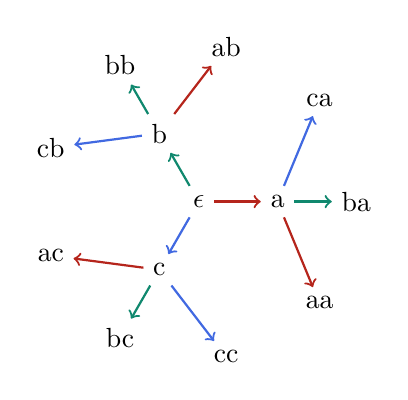
\begin{tikzpicture}
        \node (e) at (0,0) {$\epsilon$};
        \node (a) at (0:1) {a};
        \node (b) at (120:1) {b};
        \node (c) at (240:1) {c};
        \node (aa) at (-40:2) {aa};
        \node (ba) at (0:2) {ba};
        \node (ca) at (40:2) {ca};
        \node (ab) at (80:2) {ab};
        \node (bb) at (120:2) {bb};
        \node (cb) at (160:2) {cb};
        \node (ac) at (200:2) {ac};
        \node (bc) at (240:2) {bc};
        \node (cc) at (280:2) {cc};
    
        \draw[thick,->,BrickRed] (e) -- (a);
        \draw[thick,->,PineGreen] (e) -- (b);
        \draw[thick,->,RoyalBlue] (e) -- (c);
    
        \draw[thick,->,BrickRed] (a) -- (aa);
        \draw[thick,->,PineGreen] (a) -- (ba);
        \draw[thick,->,RoyalBlue] (a) -- (ca);
    
        \draw[thick,->,BrickRed] (b) -- (ab);
        \draw[thick,->,PineGreen] (b) -- (bb);
        \draw[thick,->,RoyalBlue] (b) -- (cb);
    
        \draw[thick,->,BrickRed] (c) -- (ac);
        \draw[thick,->,PineGreen] (c) -- (bc);
        \draw[thick,->,RoyalBlue] (c) -- (cc);
    \end{tikzpicture}
\end{center}
We are in a sense building up new words from old words, 
a form of induction where we have some bases case (the empty word)
and three inductive operators: prepend \code{a}, prepend \code{b}, or 
prepend \code{c}.
Notice because we only pre-pend there is no ambiguity 
in this grammar, that is, $abc$ can only mean $a(bc)$.
% Similar to the natural numbers, strings are the type 
% of another algebra, a \emph{free monoid} it will be called.
% This will become the start of a future algebra is another algebra, with one nullary operator 
% $\epsilon$ and three unary operators {\color{BrickRed}a$\Box$}, 
% {\color{PineGreen}b$\Box$}, and {\color{RoyalBlue}c$\Box$}
% being the production rules, that is the tree colors of arrows.

We can again make this computational.
\begin{Fcode}[]
data String_abc = nil
            | 'a' s:String_abc
            | 'b' s:String_abc
            | 'c' s:String_abc
\end{Fcode}
\begin{Pcode}[]
class StringABC
  case Nil extends StringABC
  case A(tail:String) extends StringABC
  case B(tail:String) extends StringABC
  case C(tail:String) extends StringABC
sealed
\end{Pcode}
    
\index{\code{<<Accept>>}}\index{grammar!accepted}
This all gets a bit tedious as we can see there is a pattern of
\code{<Character> <String>}.  So we remedy this by first we fix an alphabet
separately as its own inductive grammar and make strings that use a variable alphabet.
We need one further adaptation, since we add in new production rules in 
the services our of our main one we now indicated the productions 
that are ultimately acceptable by \code{<<Accept>>}.
\begin{Gcode}[]
<Char> ::= a | b | c | d | e
<<String>> ::= 
           | <Char> <String>
\end{Gcode}
Translated to popular coding styles this might be:
\begin{Fcode}[]
data AB = a | b
data ABC = a | b | c 
data String Char = Empty 
            | Prepend( head:Char, tail:String) 
a2 = a:String AB
a3 = a:String ABC --- a different 'a'
\end{Fcode}
We read \code{String} and now taking a parameter \code{Char}
which we could be any alphabet, but here it is given the 
choice of [a,b] and [a,b,c].
Writing \lstinline{head:Char} or \lstinline{tail:String} 
indicates that head must come from the alphabet we chose 
and tail must be some already produced string, possibly empty.
Some readers might relate to a different dialect of 
programming such as the following
\begin{Pcode}[]
class AB
  case A extends Char;  case B extends Char;
sealed
class ABC
  case A extends Char;  case B extends Char;
  case C extends Char
sealed
class String[Char]
  case Empty extends String
  case Prepend( head:Char, tail:String) extends String
sealed
a2 = new Prepend[AB](a, Empty())
a3 = new Prepend[ABC](a, Empty())
\end{Pcode}
% \end{lstlisting}
Observe the similarities with Peano's natural numbers:
\begin{align}
     2 & \defeq S(S(0)) \tag{$\mathbb{N}$}\\
 \text{\lstinline{"me"}} & \defeq \text{\lstinline{Prepend('m',Prepend('e',Empty))}}
\tag{String}
\end{align}
The left-hand sides are merely notation for what the data really is on the right.
Both the successor and the \lstinline{Prepend} are operators that generate 
new values.  Later in you shall come to know these constructions as free algebras,
but they are also foundational to programming.



\begin{remark}{Dictionaries and Sentences}
    The above examples demonstrate how the language of grammars came to 
    use terms like ``alphabet/word''. 
    In natural languages however, the building blocks of grammar are comprised of words (or
    at least syllables), as would be found in a dictionary, not an alphabet.  
    Likewise the grammar clarifies what it means to accept a string of words as a sentence,
    not what words are in the language. This offset in vocabulary better 
    approximates the tradition of languages like Chinese
    where entire words can be characters in the alphabet and strings of
    characters are sentences.
\end{remark}

\section{Elimination}
Let us now try to eliminate a string.  Recall elimination is the term used 
when we consume the structure use to introduce the data.  One example could be to imitate 
our addition of natural numbers, only now we seek an analog to ``add''
strings.  Perhaps concatenation comes to mind.  Using our $[a,b,c]$ 
alphabet ths addition could look like this.
\begin{align*}
    s+t & \defeq \begin{cases}
        t & s=\epsilon\\
        a(w+t) & s= a(w:String)\\
        b(w+t) & s= b(w:String)\\
        c(w+t) & s= c(w:String)\\
    \end{cases}
\end{align*}
Thus,
\begin{align*}
    cab+bab & = c(ab+bab)+c(a(b+bab))=c(a(b(\epsilon+bab)))\\
        & = c(a(b(bab)))=cabbab.
\end{align*}
Once more we can do the same in code by matching the pattern.
Listing~\ref{lst:peano} shows what this might look like for 
strings fixed on the alphabet [a,b,c].  Start to imagine what 
changes you would make to work with other alphabets, and 
eventually interchangeable alphabets.
\begin{lstfloat}
\begin{center}
\begin{Fcode}[]
cat:String_abc->String_abc->String_abc
cat Empty t   = t
cat 'a' tail t = 'a' (cat tail t)
cat 'b' tail t = 'b' (cat tail t)
cat 'c' tail t = 'c' (cat tail t)
\end{Fcode}
\begin{Pcode}[]
def cat(s,t:String_abc):String_abc =
  match s with 
    Empty() => t
    A(tail)=> A(cat(tail,t))
    B(tail)=> B(cat(tail,t))
    C(tail)=> C(cat(tail,t))
\end{Pcode}
\end{center}
\caption{Concatenation of strings over the alphabet [a,b,c] is a variation on 
Peano's addition of natural numbers.}
\label{lst:peano-elim}
\end{lstfloat}
    
% This algorithm remains predictable because of what we assumed about 
% primitive recursion.  That is $m+0$ is defined and if $m+k$ is defined 
% then $m+S(k)\defeq S(m+k)$ is therefore defined.  This is what is 
% known as \emph{recursion}.  It hinges on the fact that the proper 
% \[    P(n) :\equiv m+n \text{ defined}
% \]
% we want is known at step $k$, we write $P(k)$, and so we can 
% use that knowledge to deduce the $m+S(k)$ is defined, in other wards $P(S(k))$ follows.
% \begin{gather*}
%     \begin{array}{rl}
%     P(0)& \\
%     P(k) & \Rightarrow P(k+1)\\
% \hline 
% \forall n:\mathbb{N} & P(n).
%     \end{array}
% \end{gather*}
% This is sometimes known as the principle of induction.  It is more of a program than 
% an assumption of fact.  When we have a $n$ we want to confirm $m+n$ is defined for,
% say $n=SS0$, then we simply apply the rules given repeatedly:
% \[
%     m+SS0=S(m+S0)= SS(m+0)=SS(m)
% \]
% By rule \code{S<Nat>} we get that $SS(m):\mathbb{N}$.  As expected it added two strokes to the 
% tally.   This process of consuming the information given to introduce $n:\mathbb{N}$ is known 
% as \emph{elimination}.   We will see several examples introduction 
% and elimination patterns. 

% If we stand back to observe the entire process, grammars allow us to introduce numbers, 
% such as $2\defeq SS0:\mathbb{N}$.  Then when we have $2:\mathbb{N}$ we can 
% use the data behind its introduction (here two successors and a $0$) as instructions 
% to follow when producing a new outcome, perhaps a new type of data.  This is known 
% as \emph{eliminating} the introduction.  We will see several examples introduction 
% and elimination patterns. 

% \subsection{Type rules}
% We are engaged in forming a type of data, natural numbers.  Some times 
% of data will depend on others, for example tuples $\mathbb{N}^k$ depend on 
% $k$.  So even in the form of types we need to pause and 


% If we break down the 
% steps we first had to give the type a name, 
% If we break this process down here are the summary points.  Note that we use Frege's 
% notation where symbols $p_1,\ldots,p_n$ that lead to symbols $q$ are separated by 
% $\vdash$, so $p_1,\ldots,p_n\vdash q$, which is also often written 
% \begin{align*}
%     \frac{p_1,\ldots,p_n}{q}\qquad 
%     \begin{array}{c}
%         p_1\\
%         \vdots \\
%         p_n\\
%     \hline 
%         q 
%     \end{array}
% \end{align*}
% Note that if nothing is required to lead to $q$ we can write $\vdash q$.
% The symbol $\vdash$ is known formally as \emph{entailment} and while it may 
% appear at first like an implication, it is here being used more in the role of 
% defining rules.
% \begin{gather}
%     \tag{$\form{\mathbb{N}}$}
%     \vdash \mathbb{N}:Type\\
%     \tag{$\intro{\mathbb{N}}$}
%     \vdash 0:\mathbb{N} 
%     \qquad \frac{k:\mathbb{N}}{S(k):\mathbb{N}}\\
%     \tag{$\elim{\mathbb{N}}$}
%     \begin{array}{rl}
%         n &:\mathbb{N}\\
%         P(k) &\vdash P(S(k))\\
%     \hline 
%         P(n)
%     \end{array}
% \end{gather}

% \subsection{Wrapping up errors}
% \begin{center}
% \begin{minipage}{0.35\textwidth}
% \begin{Fcode}
% data Maybe B = 
%     | Just (b:B)  
%     | None 
% \end{Fcode}
% \end{minipage}
% ~
% \begin{minipage}{0.64\textwidth}
% \begin{Pcode}
% class Option[B]
%     case Some(b:B) extends Option[B]
%     case None() extends Option[Any]
% sealed
% def wrap(f:A->B):f:A->Option[B] = 
%     a ->
% \end{Pcode}
% \end{minipage}
% \end{center}
    